\documentclass[12pt, a4paper]{article}
\usepackage[utf8]{inputenc}
\usepackage[T1]{fontenc}
\usepackage[slovene]{babel}
\usepackage{lmodern}
\usepackage{amsmath}
\usepackage{eurosym}
\usepackage{amsfonts}
\usepackage{hyperref}
\usepackage{graphicx}
\usepackage{tikz}


\usepackage{enumerate}
\setlength{\parindent}{0mm}

\newcommand{\novukaz}[2]{\underline {#1} \textit{#2}}

\newcounter{stevec}

\newenvironment{novookolje}[2]{\stepcounter{stevec} #1 #2 \thestevec}{}


\begin{document}
\begin{titlepage}
\begin{center}

\large
Univerza v Ljubljani\\
\normalsize
Fakulteta za matematiko in fiziko\\

\vspace{3 cm} 

\large
Eva Deželak, Žan Jarc in Ines Šilc\\

\vspace{0.5cm}
\LARGE
\textbf{PRORAČUN REPUBLIKE SLOVENIJE}

\vspace{0.5 cm}
\normalsize


\vspace{1.5cm}
\normalsize
Mentor: doc. dr. Matjaž Črnigoj

\vspace{3cm}


\vfill

\large Ljubljana, 2019

\end{center}
\end{titlepage}



\newpage
\section*{Povzetek}
\hspace*{5mm} Proračun Republike Slovenije je akt države, s katerim so predvideni vsi prihodki in drugi prejemki ter odhodki in drugi izdatki države za eno leto. Proračun sprejme Državni zbor po posebnem, predpisanem postopku. \\
\hspace*{5mm} Proračun Republike Slovenije se deli na tri večje dele in sicer: splošni del proračuna, posebni del proračuna in načrt razvojnih programov. Splošni del proračuna vsebuje bilanco prihodkov in odhodkov, račun finančnih terjatev in naložb ter račun financiranja. Posebni del proračuna pomeni vsebino porabe javnofinančnih sredstev v finančnih načrtih posameznih proračunskih uporabnikov oziroma skupin proračunskih uporabnikov in vključuje odhodke in druge izdatke delovanja predstavljene po politikah, glavnih programih in podprogramih.  V načrtu razvojnih programov se odhodki načrtujejo po strukturi programske klasifikacije, posameznih ukrepih in projektih ter virih financiranja po posameznih letih za celovito izvedbo projektov in ukrepov. \\
\hspace*{5mm} Postopek priprave in sprejemanja državnega proračuna delimo na vladno in parlamentarno fazo. Prvi del opravi vlada Republike Slovenije, ki nato posreduje predloge proračunov v Državni zbor RS. Nato v državnem zboru sledi obravnava in sprejemanje državnega proračuna. V Sloveniji se praviloma sprejemata proračuna za dve leti vnaprej, torej za prihodnje leto in za leto, ki mu sledi. \\
\hspace*{5mm} Prispevki za pokojninsko in invalidsko zavarovanje se skozi leta povečujejo, kar je pričakovano, glede na starost prebivalstva. Velik problem nam predstavlja demografija, vse več imamo starejših ljudi ter ljudi nad 50 let z nizko stopnjo aktivnosti. Dolgoročna vzdržnost je vprašljiva. Predlogi v novi pokojninski reformi niso ugodni za proračun, saj omogočajo upokojitev veliko več osebam kot bi bilo priporočljivo. \\
\hspace*{5mm} V primerjavi z drugimi državami ima Slovenija nizko upokojitveno starost in visok delež ljudi nad 50 let, ki dobivajo pokojnino.\\
\hspace*{5mm} Zaradi trenutnega ugodnega gospodarskega stanja se na prvi pogled zdi slovenski pokojninski sistem še dokaj stabilen, vendar se lahko to hitro spremeni.



\newpage

\tableofcontents
\vspace{20mm}

\newpage
\section[Uvod]{Uvod}
\hspace*{5mm} V seminarski nalogi bomo predstavili proračun Republike Slovenije. Najprej se bomo osredotočili na to, kaj sploh je proračun, kako je sestavljen in kako poteka njegova priprava, ter kako poteka njegovo izvrševanje.\\
\hspace*{5mm} Analizirali bomo nekaj sprememb, ki so se zgodile v poračunu Republike Slovenije med leti 2015 do 2019. Osredotočili se bomo predvsem na dele proračuna, kjer so bile opazne spremembe, saj večina proračuna ostaja dokaj konstantna. Deli, kjer so opazne spremembe so predvsem pri davkih na dohodek, premičnine, nepremičnine in finančnega premoženje.\\
\hspace*{5mm} Nato bomo preverili različne vplive demografije na proračun. Predvsem se bomo osredotočili na staranje prebivalstva in kako se država spopada s tem. Analizirali bomo prispevke za pokojninsko in invalidsko zavarovanje in prispevke delodajalcev za zdravstveno zavarovanje, torej na splošno vse prispevke za pokojninski sklad. Omenili bomo kakšni so sploh zakoni o financiranju pokojnin iz državnega proračuna in primerjali, kako se v drugih državah soočajo s staranjem prebivalstva in kakšne so sploh razmere tam.\\
\hspace*{5mm} Navedli bomo nekaj predlogov za spremembe pokojninskega sistema v Sloveniji in poskušali razmisliti, kako bi lahko te spremembe vplivale na podjetja in na delavce na splošno.\\
\hspace*{5mm} V predzadnjem delu bomo analizirali pokojninske transferje v Sloveniji in v ostalih državah, ter primerjali razmere.\\
\hspace*{5mm} Za konec pa si bomo pogledali še nekaj možnih projekcij za prihodnost in poskušali ugotoviti katere predpostavke so ključne pri načrtovanju projekcij.
\\
\newpage

\section[Splošno o proračunu RS]{Splošno o proračunu RS}
\hspace*{5mm} V preteklosti je izraz "budžet"~v slovenščino prodrl iz angleškega jezika, kjer je prvotno predstavljal torbo, v kateri je imel kralj spravljen denar za javne izdatke. \\
\hspace*{5mm} Danes se izraz "proračun"~uporablja le za letni načrt prihodkov in odhodkov družbeno - političnih skupnosti (npr. državni, občinski proračun).\\
\hspace*{5mm}
Proračun Republike Slovenije je akt države, s katerim so predvideni vsi prihodki in drugi prejemki ter odhodki in drugi izdatki države za eno leto. Proračun sprejme Državni zbor po posebnem, predpisanem postopku.\\
\hspace*{5mm}
Državni proračun je pomemben instrument, ki ga ima vlada na voljo pri izvajanju večletne makroekonomske politike, katere cilj je zagotavljanje stabilnih javnih financ in pospeševanje gospodarskega ter družbenega razvoja. Temeljne naloge pri upravljanju proračuna so uresničitev proračuna v okvirih in za namene, kot je bil sprejet, njegovo pravočasno in fleksibilno prilagajanje spremenjenim fiskalnim okoliščinam ter uresničevanje v proračunu zastavljenih družbenih in gospodarskih ciljev. Vir: [\ref{Splošno o proračunu}]

\subsection[Sestavni deli proračuna]{Sestavni deli proračuna}
\subsubsection[Splošno del proračuna]{Splošni del proračuna}
Splošni del proračuna vključuje bilanco prihodkov in odhodkov, račun finančnih terjatev in naložb ter račun financiranja.
\begin{itemize}
\item V \textbf{bilanci prihodkov in odhodkov} se izkazujejo prihodki, ki obsegajo tekoče prihodke (davčne in nedavčne prihodke), kapitalske prihodke, prejete donacije ter transferne prihodke iz drugih blagajn javnega financiranja. Na strani odhodkov pa se izkazujejo odhodki, ki zajemajo tekoče odhodke, tekoče transfere, investicijske odhodke ter investicijske transfere.

\item \textbf{Račun finančnih terjatev} zajema na strani izdatkov tiste tokove izdatkov, ki za državo nimajo značaja odhodkov (to je nepovratno danih sredstev), pač pa imajo bodisi značaj danih posojil finančnih naložb oziroma kapitalskih vlog države v javna in zasebna podjetja, banke oziroma druge finančne institucije. Plačila imajo za rezultat nastanek finančne terjatve države (ali občine) do prejemnika teh sredstev ali pa vzpostavitev oziroma povečanje kapitalskega deleža države v lastniški strukturi prejemnikov teh sredstev. V okviru te skupine izdatkov se izkazujejo tudi plačila zapadlih jamstev države finančnim institucijam ali drugim upnikom, s čimer nastane terjatev države (regresna pravica) do glavnega dolžnika (osebe, za katero je država jamčila). Na strani prejemkov pa so v tem računu izkazani tokovi prejemkov, ki nimajo značaja prihodkov, pač pa so to sredstva iz naslova prejetih vračil posojenih sredstev države oziroma prejetih sredstev iz naslova prodaje kapitalskih deležev države v podjetjih, bankah in drugih finančnih institucijah.

\item V \textbf{računu financiranja} se izkazujejo tokovi zadolževanja in odplačil dolgov, povezanih s servisiranjem dolga države, oziroma s financiranjem proračunskega deficita, to je salda bilance prihodkov in odhodkov ter računa finančnih terjatev in naložb. Zadolževanje je razčlenjeno na najemanje domačih in tujih kreditov ter na sredstva, pridobljena z izdajo državnih vrednostnih papirjev na domačem in tujem trgu. Odplačila dolga pa so razčlenjena na odplačila domačih in tujih kreditov ter odplačila glavnice zapadlih državnih vrednostnih papirjev. V računu financiranja se kot saldo izkazujejo tudi spremembe stanja denarnih sredstev na računih med proračunskim letom.
\end{itemize}

\subsubsection[Posebni del proračuna]{Posebni del proračuna}
\hspace*{5mm} Posebni del proračuna pomeni vsebino porabe javnofinančnih sredstev v finančnih načrtih posameznih proračunskih uporabnikov oziroma skupin proračunskih uporabnikov in vključuje odhodke in druge izdatke delovanja predstavljene po politikah, glavnih programih in podprogramih. 

\subsubsection[Načrt razvojnih programov]{Načrt razvojnih programov}
\hspace*{5mm} V načrtu razvojnih programov se odhodki načrtujejo po strukturi programske klasifikacije, posameznih ukrepih in projektih ter virih financiranja po posameznih letih za celovito izvedbo projektov in ukrepov. Načrt razvojnih programov se izdela za obdobje celotnega trajanja v načrt vključenih ukrepov in projektov. V proračunu se prikaže po ukrepih, skupinah projektov in projektih ter virih sredstev za njihovo izvedbo. Vir: [\ref{Sestavni deli}]

\subsection[Priprava proračuna]{Priprava proračuna}
\hspace*{5mm} Postopek priprave in sprejemanja državnega proračuna delimo na vladno in parlamentarno fazo:
\begin{enumerate}
\item postopek priprave predloga državnega proračuna in potrditve na vladi,
\item postopek obravnave in sprejemanja državnega proračuna v državnem zboru.
\end{enumerate}
\hspace*{5mm} V Sloveniji se praviloma sprejemata proračuna za dve leti, za prihodnje leto (t+1) in leto, ki temu sledi (t+2). S tem se zagotavlja kontinuirano financiranje države za dve leti. Zato tečeta postopka za pripravo predloga sprememb proračuna za prihodnje leto in pripravo predloga proračuna za leto, ki sledi prihodnjemu letu, sočasno. Vir: [\ref{Priprava proračuna}]

\subsection[Izvrševanje proračuna]{Izvrševanje proračuna}
\hspace*{5mm} Izvrševanje proračuna obsega vse postopke in aktivnosti, ki jih je treba opraviti za to, da se realizira sprejeti proračun tako na nivoju proračuna kot celote kot na ravni posameznega finančnega načrta. Izvrševanje proračuna se prične z uveljavitvijo proračuna in traja do konca proračunskega leta, ko je treba poročati o izvršitvi proračuna in v ta namen pripraviti zaključni račun proračuna. Vir: [\ref{Izvrševanje proračuna}]

\newpage
\section[Analiza nekaterih sprememb proračuna v letih od 2015 do 2019]{Analiza nekaterih sprememb proračuna v letih od 2015 do 2019}

\hspace*{5mm} Najprej si oglejmo različne davke. Zanimivo je, da je bil davek na nepremičnine uveden samo v letu 2015, zato so podatki o prihodkih tega davka prisotni samo za leto 2015. Istega leta so bili tudi najvišji prihodki iz davka na finančno premoženje in davka na premičnine. Spodnji graf prikazuje prihodke davka na premičnine in davkov na promet nepremičnin ter na finančno premoženje.
\begin{figure}[h!]
\centering
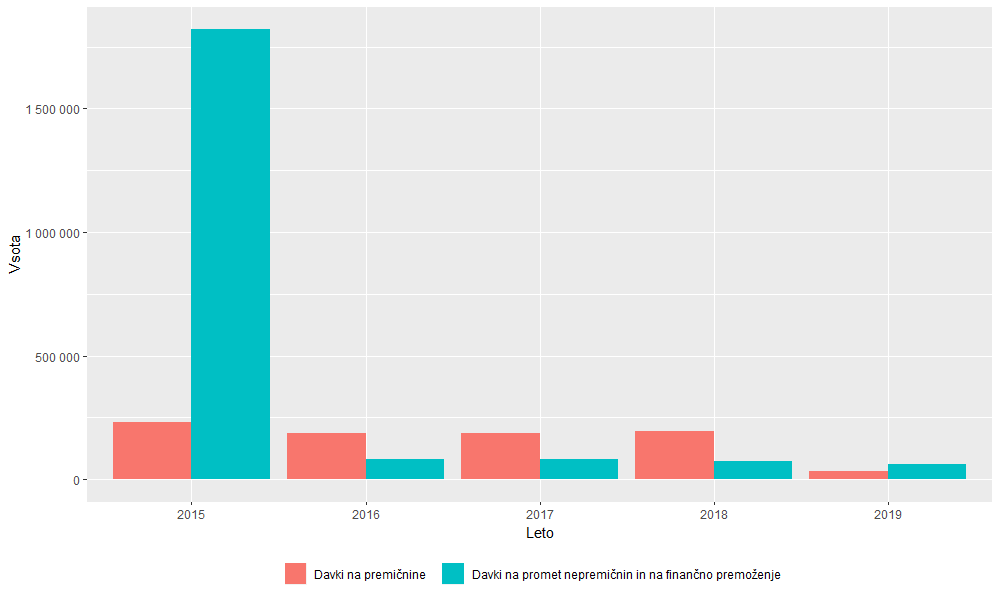
\includegraphics[width = 14 cm]{davki_na_premozenje_graf.png}
\caption{Prispevki davkov na premičnine in na promet nepremičnin}
\label{Slika 1}
\end{figure}

\hspace*{5mm} Druga večja sprememba se pojavi pri davku na dohodek pravnih oseb in dohodnini. Opazimo zelo velik skok pri prispevkih od dohodnin iz leta 2015 na leto 2019 in sicer za približno četrt milijona. Prav tako se višajo prispevki od davkov pravnih oseb, za malo manj kot pol milijona. Pri obeh davkih opazimo približno enako počasno rast v letih 2015 do 2018 in nato velik skok. Spodnji graf prikazuje davek od dohodkov pravnih oseb, dohodnino in druge davke na dohodek in dobiček v proračunu RS.
\begin{figure}[h!]
\centering
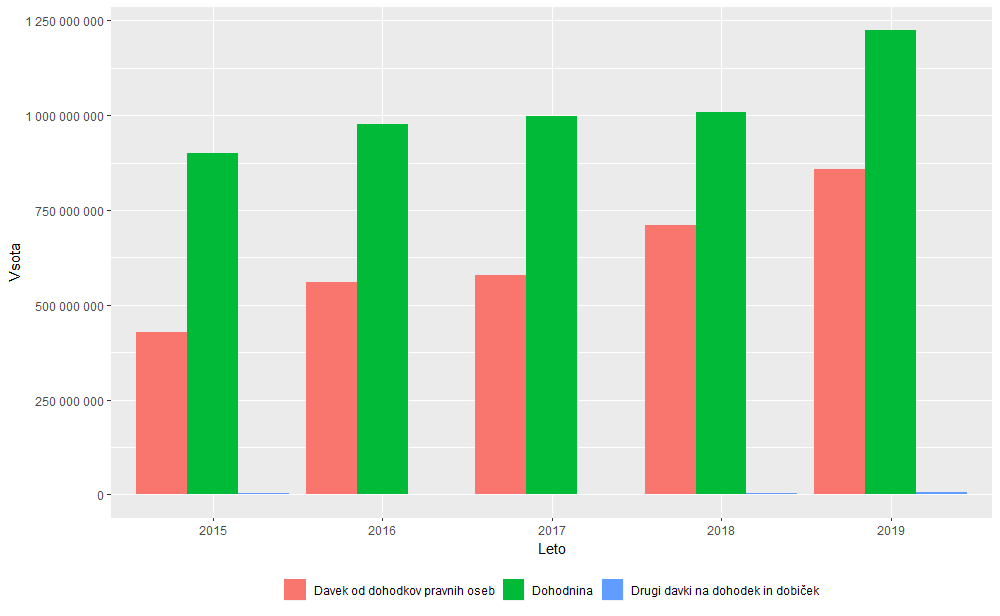
\includegraphics[width = 14 cm]{davki_na_dohodek_in_dobicek_graf.png}
\caption{Prispevki davkov na dohodek in dobiček}
\label{Slika 2}
\end{figure}

\newpage
\section[Demografski vplivi na proračun]{Demografski vplivi na proračun}
\subsection[Pokojnine]{Pokojnine}
\hspace*{5mm} V proračunu RS se prispevki za pokojninski sklad kažejo v dveh kategorijah. Prva kategorija so prispevki za pokojninsko in invalidsko zavarovanje, druga kategorija pa so premije kolektivnega dodatnega pokojninskega zavarovanja na podlagi ZKDPZJU\footnote{Zakon o kolektivnem dodatnem pokojninskem zavarovanju za javne uslužbence}, ki je začel veljati leta 2003. Spodnji graf prikazuje obe kategoriji ter prispevke za zdravstveno zavarovanje v proračunu od leta 2015 do leta 2019.
\begin{figure}[h]
\centering
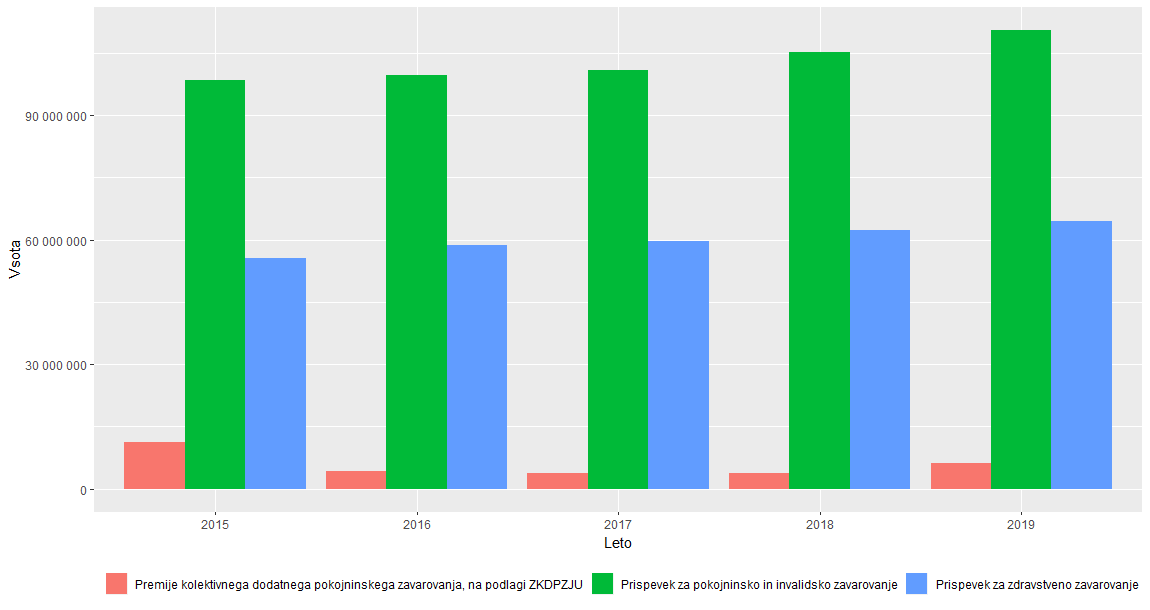
\includegraphics[width = 14 cm]{prispevki_delodajalcev_za_socialno_varnost_graf.png}
\caption{Prispevki za pokojninski sklad v proračunu RS}
\label{Slika 3}
\end{figure}

\hspace*{5mm} Vidimo, da se prispevki za pokojninsko in invalidsko zavarovanje povečujejo, kar je tudi pričakovano glede na sestavo slovenskega prebivalstva, medtem ko je bila premija dodatnega pokojninskega zavarovanja najvišja leta 2015. Da razumemo, zakaj se prispevki za pokojnine povečujejo, moramo poznati demografsko sestavo prebivalstva v Sloveniji. Oktobra 2018\footnote{Zadnji možni podatki o prebivalstvu Slovenije}, je bila povprečna starost prebivalcev 43,3 leta, medtem ko se je delež prebivalcev starih nad 65 let od leta 2015 povečal iz 17.9\% do 19.4\% [\ref{Prebivalstvo Slovenije}]. V Sloveniji imamo tudi zelo nizko stopnjo aktivnosti ljudi nad 50 let. Dolgoročna vzdržnost je tu vprašljiva, saj vlada vsako leto namenja velike transferje iz proračuna za pokojnine. Nova zakonodaja je že omejila možnosti predčasne upokojitve in s tem povzročila, da se veliko manj ljudi upokojuje predčasno, kar je dobro za proračun. V novi pokojninski reformi pa se pripravljajo predlogi, ki niso tako ugodni za proračun, saj naj bi predlagali, da bi se lahko oseba z dopolnjenimi 40-imi leti delovne dobe, upokojila kadarkoli po 60 letu starosti. V primerjavi z drugimi državami ima Slovenija nizko povprečno upokojitveno starost.

\subsubsection[Financiranje pokojnin iz državnega proračuna]{Financiranje pokojnin iz državnega proračuna}

\hspace*{5mm} Zakon o pokojninskem in invalidskem zavarovanju v dveh členih povzema naloge državnega proračuna pri financiranju pokojninskega zavarovanja, to sta člena 162. in 163. [\ref{ZPIZ2}]:
\begin{itemize}
	\item \textbf{162. člen}: Sofinanciranje iz državnega proračuna: Republika Slovenija iz državnega proračuna in iz drugih virov zagotavlja sredstva za pokrivanje razlike med prihodki zavoda iz prispevkov in iz drugih virov ter odhodki zavoda.
	\item \textbf{163. člen}: Zagotavljanje likvidnosti zavoda: Če zavodu primanjkuje likvidnih sredstev za izpolnitev obveznosti za izplačilo pokojnin in drugih obveznosti ter za kritje morebitnega primanjkljaja med prihodki in odhodki v posameznem koledarskem letu, mu Republika Slovenija iz državnega proračuna zagotovi potrebna sredstva.
\end{itemize}

\hspace*{5mm} Namen dodatnega pokojninskega zavarovanja je, da že v delovni dobi posameznik poskrbi za dodaten vir dohodka, ki bo nadomestil izpad dohodka iz obveznega pokojninskega zavarovanja zaradi negativnega demografskega vpliva.

\hspace*{5mm} Pomembne novosti v dodatnem pokojninskem zavarovanju, s sprejetjem drugega zakona o  pokojninskem in invalidskem zavarovanju, vir: [\ref{Novosti ZIPZ2}]:
\begin{itemize}
	\item Vsi zaposleni so po svoji izbiri vključeni v kolektivno dodatno pokojninsko zavarovanje, kdor ne želi biti vključen, mora delodajalcu podati pisno izjavo.
	\item Mlajšim zavarovancem bo zagotovljen manj konzervativen način varčevanja.
	\item V kolektivno dodatno zavarovanje se v skladu z novo zakonodajo lahko vključijo tudi samostojni podjetniki in pretežni lastniki podjetja\footnote{Za pretežnega lastnika velja oseba, ki ima v lasti vsaj 25\% podjetja}.
\end{itemize}




\subsubsection[Primerjava z drugimi državami]{Primerjava z drugimi državami}
\hspace*{5mm} Leta 2012 je bilo povprečno leto, pri katerem je državljan prejemal prvo pokojnino v Sloveniji enako 56.6, medtem ko je bilo mediansko leto enako 57. Graf \ref{Slika 4} prikazuje leto prve pokojnine pri primerljivih državah.
\begin{figure}[h]
\centering
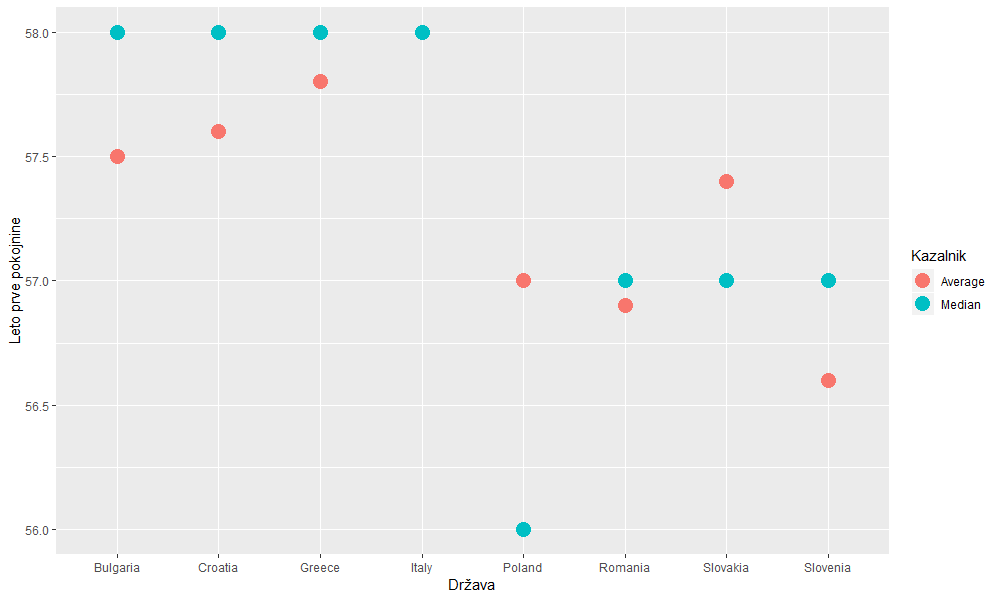
\includegraphics[height = 7 cm]{leto_prve_pokojnine.png}
\caption{Leto prve pokojnine, vir: [\ref{Eurostat pokojnine}]}
\label{Slika 4}
\end{figure}
Slovenijo lahko torej primerjamo z Albanijo v primeru leta prve pokojnine, vendar je njihova sestava prebivalstva drugačna, saj predstavljajo ljudje nad 65 let le 13.2\%, medtem ko je ta delež v Sloveniji enak 15.1\%, vir: [\ref{Struktura prebivalstva}]. Mediansko leto prve pokojnine je enako še na Slovaškem, medtem, ko je povprečno leto prve pokojnine v Sloveniji med nižjimi v Evropi.

\begin{figure}[h!]
\centering
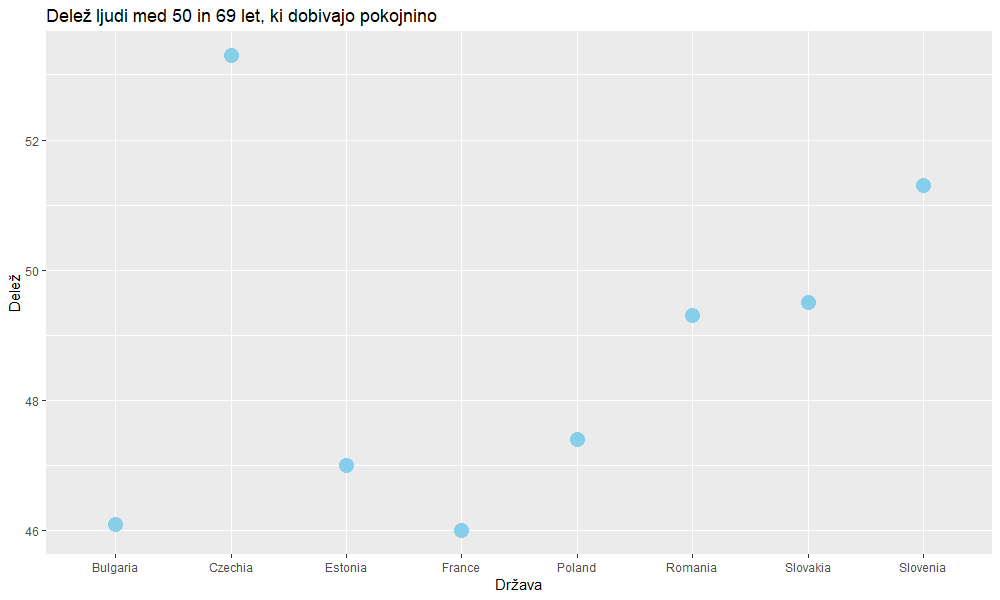
\includegraphics[width = 13 cm]{graf_procentualno_pokojnina.png}
\caption{Delež ljudi med 50 in 69 let, ki dobivajo pokojnino, vir: [\ref{Eurostat pokojnine procentualno}]}
\label{Slika 5}
\end{figure}

\hspace*{5mm} Poglejmo si še delež ljudi med 50 in 69 let, ki dobivajo pokojnino. To prikazuje graf \ref{Slika 5}. Ta podatek je v Sloveniji 51.3\%, leži med Češko, kjer je delež 53.3\% in Slovaško 49.3\%. Delež starejših oseb je na Češkem 19\%, na Slovaškem pa 15.1\%.

\newpage
\subsection[Predolgi za spremembe pokojninskega sistema v Sloveniji]{Predlogi za spremembe pokojninskega sistema v Sloveniji}

\hspace*{5mm} Trenutna zakonodaja že ponuja veliko spodbud za podaljšanje delovne dobe. Za vsako dodatno leto dela se odmerjeni odstotek pokojnine poveča za 4\%, vendar največ za 3 leta. Imamo tudi možnost prejemanja dodatne pokojnine poleg plače, dobiva še 20\% pokojnine. Teh 20\% je obdavčenih neto, torej dobi oseba dodatnih 10\%. Negativne spodbude pa daje s tem, da omeji možnost predčasnih upokojitev: za vsak mesec manjkajoče starosti do 65 let se pokojnina zmanjša za 0.3\%.

\hspace*{5mm} Veliko več denarja za pokojnine bi lahko prišlo iz dodatnega pokojninskega zavarovanja, zato se splača ljudi spodbuditi k temu, da več svojih prihrankov namenijo dodatnemu pokojninskemu zavarovanju. Vlada bi lahko tako obliko varčevanja stimulirala s primernimi davčnimi olajšavami.\par

\hspace*{5mm} Predčasne upokojitve lahko zmanjšamo tudi z zaposlovanjem starejših ljudi, saj se le-ti z leti počutijo, kot da ne napredujejo v skladu s tehnologijo in so zato nezaželjeni na delovnih mestih. Vlada bi morala nameniti dovolj sredstev z preizobraževanje starejših državljanov in poskrbeti, da so zadovoljni z novimi delovnimi mesti, na katerih se morajo počutiti sprejete.
\\
\\
\hspace*{5mm} Negativna posledica zgornjih navedb za podjetja bo predvsem to, da se bo zviševal dodatek za delovni dobo, ki ga podjetja izplačujejo pri plačah svojim zaposlenim, saj se le ta viša s starostjo zaposlenih. Poleg tega tehnologija zelo hitro napreduje in ji človek s starostjo težje sledi. Zato bo delodajalec moral vlagati v  dodatna izobraževanja za starejše, če bo želel da bodo tudi ti v koraku s tehnologijo in vsem, kar potrebujejo pri svojem delu. To bo od podjetja zahtevalo dodatne stroške. Pogosteje bi lahko prihajalo do napak oziroma nenatančnosti, tudi zaradi same starosti zaposlenega, saj se s starostjo zmanjšujejo nekatere telesne funkcije. To je predvsem odvisno od narave dela, pri fizičnih delih bi se to bolj poznalo. S starostjo se povečajo možnosti za določene bolezni oziroma težave s počutjem, kar bi podjetju prineslo dodatne stroške bolniške odsotnosti. Torej podjetja bi lahko s starejšimi zaposlenimi imela večji strošek za nižjo produktivnost.

\hspace*{5mm} Po drugi strani pa ima običajno starejši delavec več delovnih izkušenj in določenega znanja, ki si ga je pridobil v času svoje delovne dobe. V kolikor bi znal delodajalec izkoristiti te njegove potenciale, bi lahko podjetju s svojim znanjem delavec veliko doprinesel, tudi na primer s prenosom znanja na mlajše, oziroma nove delavce, novimi predlogi in izboljšavami pri delu. Hkrati pa je podjetje, ki zaposli starejše ljudi, upravičeno do olajšave za DDPO (davek na dohodek pravnih oseb) - po zakonu namreč velja, da so podjetja upravičena do olajšave za zaposlovanje, če na novo zaposlijo osebo, ki je starejša od 55 let, ki je prej 6 mesecev prijavljena na Zavodu za zaposlovanje; in sicer je olajšava v višini 45\% plače te osebe. 

\newpage
\section[Analiza pokojninskih transferjev v Sloveniji in ostalih državah]{Analiza pokojninskih transferjev v Sloveniji in ostalih državah}
\subsection{Analiza pokojninskih transferjev v Sloveniji}
\hspace*{5mm} Analizo slovenskih pokojninskih transferjev bomo naredili za med leti 2015 in 2019. 

\begin{figure}[h]
\centering
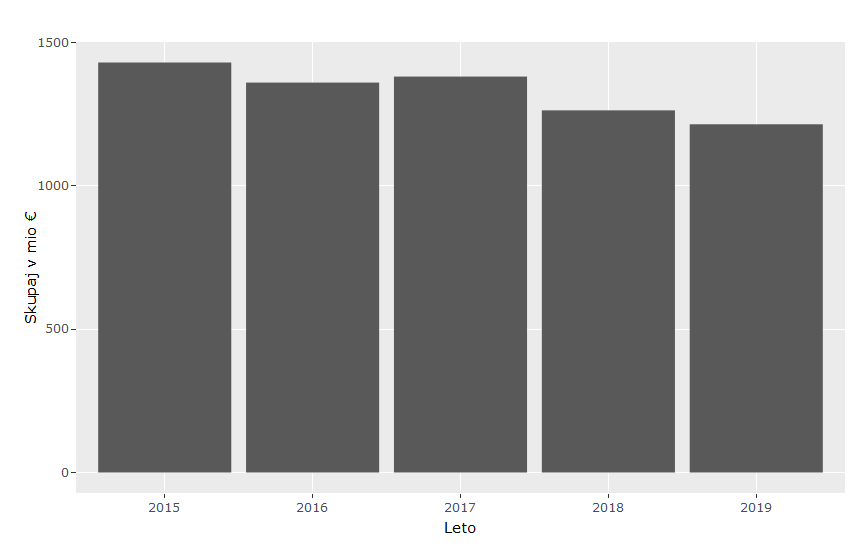
\includegraphics[height = 8 cm]{pokojnine_slovenija.png}
\caption{Pokojnine v Sloveniji, vir: [\ref{Splošno o proračunu}]}
\label{Slika 6}
\end{figure}
\hspace*{5mm} Kot lahko vidimo, država skoraj vsako leto nameni manj odhodkov za poravnavo pokojninskega računa. Na prvi pogled se zdi vse običajno, vendar če upoštevamo demografijo in napovedi o spremembi le-te, bo slovenski pokojninski sistem dokaj kmalu potreboval tehten razmislek in spremembo. Za zdaj pa nas rešuje ugodna gospodarska klima.

\begin{figure}[t!]
\centering
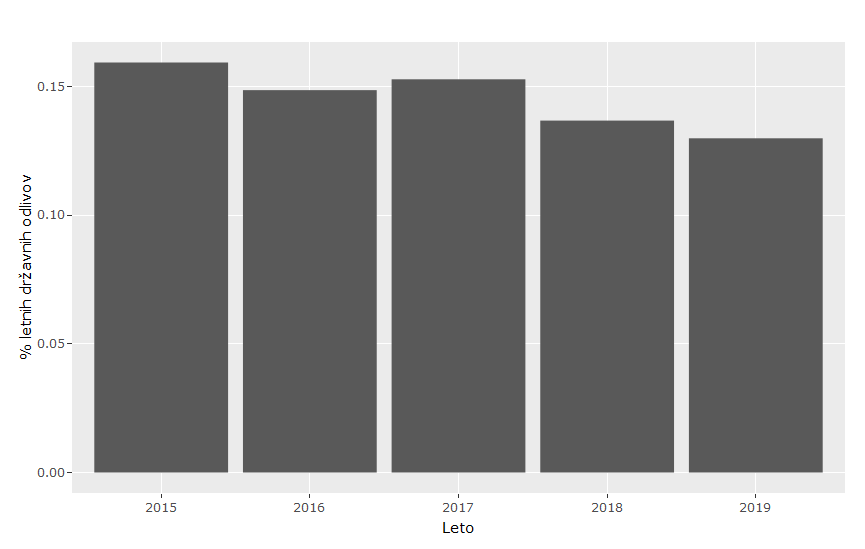
\includegraphics[height = 7 cm]{pokojnine_procentualno.png}
\caption{Delež proračunskih odlhodkov namenjen pokojninam, vir: [\ref{Splošno o proračunu}]}
\label{Slika 7}
\end{figure}

\begin{figure}[h!]
\centering
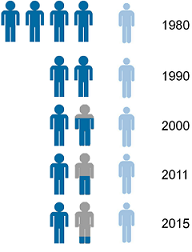
\includegraphics[height = 7 cm]{razmerje_med_zaposlenimi_in_upokojenimi_2015.png}
\caption{Razmerje med zaposlenimi in upokojenimi, vir: [\ref{BDP na prebivalca}]}
\label{Slika 8}
\end{figure}

\hspace*{5mm} Iz slike \ref{Slika 8} se zelo jasno vidi, da so bili v letu 1980 v Sloveniji na enega upokojenega državljana štirje zaposleni, razmerje pa se je skozi leta drastično slabšalo. Največji upad zaposlenih na enega upokojenca je viden iz leta 1980 na leto 1990. Do leta 2015 pa je to razmerje že skoraj en zaposleni na enega upokojen, kar je precej zaskrbljujoče.

\newpage

\newpage
\subsection{Analiza pokojninskih transferjev v drugih državah in primerjava s Slovenijo}
\hspace*{5mm} Kot v prejšnjem poglavju bomo poleg Slovenije analizirali še pokojninske transferje Bolgarije, Češke, Estonije, Poljske, Romunije in Slovaške.

\begin{figure}[h!]
\centering
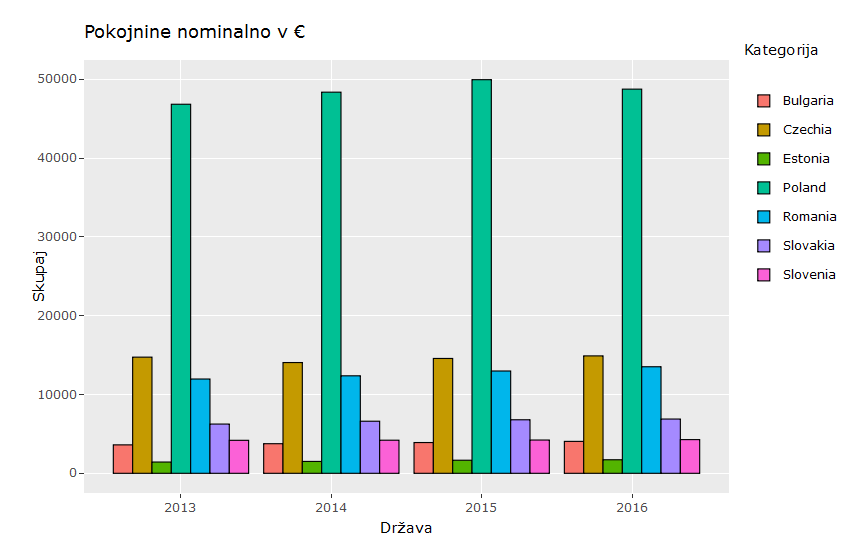
\includegraphics[height = 6 cm, width = 12 cm]{pokojnine_nominalno.png}
\caption{Pokojnine nominalno v \euro, vir: [\ref{Pokojninski transferji v državah}]}
\label{Slika 9}
\end{figure}

\hspace*{5mm} Res, da so nominalne številke pri analizi ponavadi brezpredmetne, vendar lahko pri hitrem pregledu grafa opazimo, da ima Estonija zelo malo pokojninskih transferjev. Estonija ima okoli 1,3 milijonov prebivalcev, torej malce več kot polovico kot jih ima Slovenija, za pokojninske transferje pa namenja skoraj trikrat manj. 

\begin{figure}[h!]
\centering
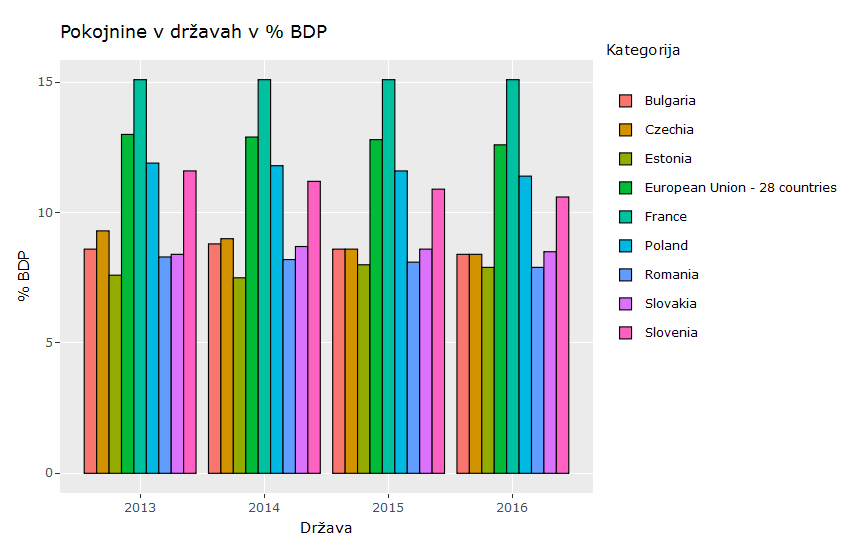
\includegraphics[height = 6 cm, width = 12 cm]{pokojnine_bdp.png}
\caption{Pokojnine v državah v \% BDP, vir:[\ref{Pokojninski transferji v državah}]}
\label{Slika 10}
\end{figure}


\begin{figure}[h!]
\centering
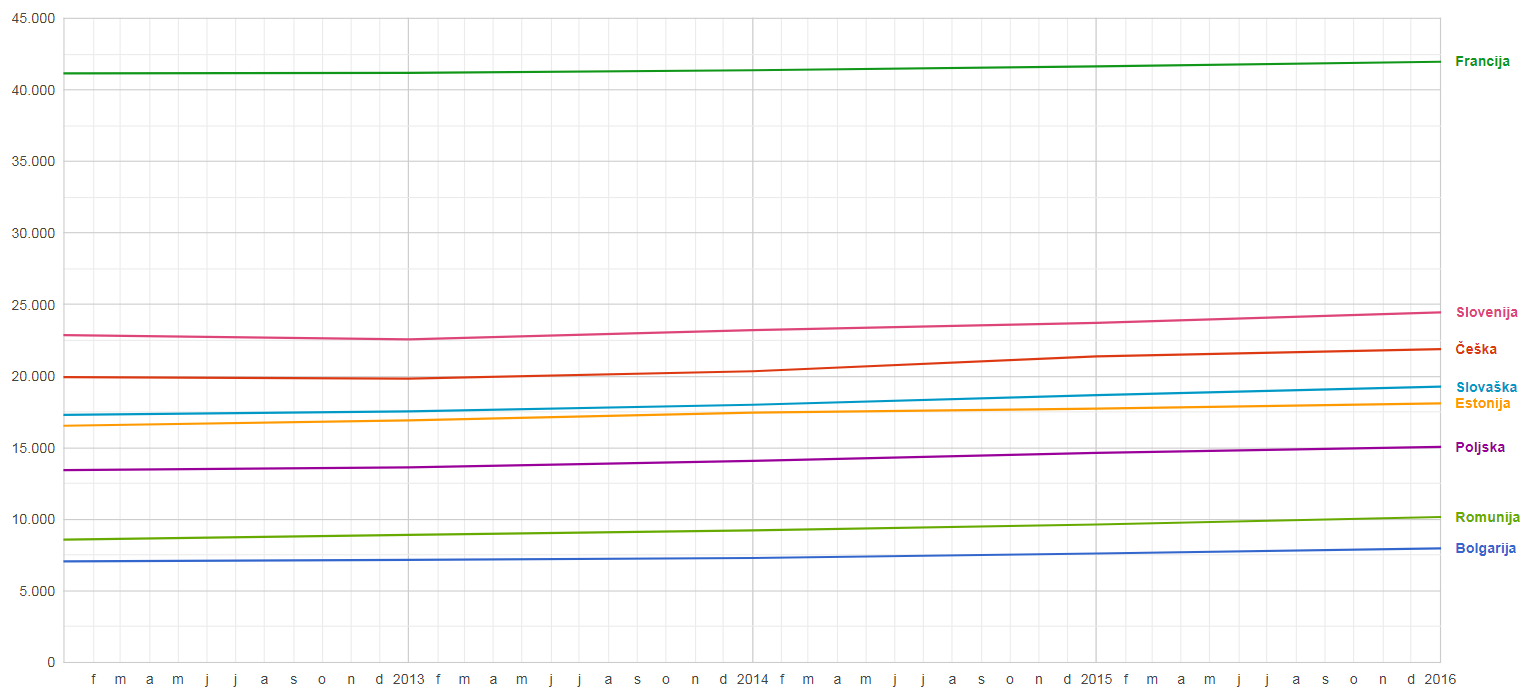
\includegraphics[width = 14 cm]{bdp_per_capita.png}
\caption{BDP na prebivalca, vir: [\ref{BDP na prebivalca}]}
\label{Slika 11}
\end{figure}

\newpage
\hspace*{5mm} V tem grafu smo dodali še Francijo za 'zahodni' benchmark. Opazimo, da je Slovenija v tej rubriki daleč pred ostalimi državami nekdanjega vzhodnega bloka, izključujoč Poljsko. Se je pa slovensko razmerje med pokojninskimi transferji in BDP-jem skozi leta 2013 - 2016 vsako leto zmanjšalo. Če to primerjamo s podatki o slovenskem BDP-ju na prebivalca, ki je med leti 2013 in 2016 rastel, ugotovimo, da so pokojnine v tem času res stagnirale, oziroma se niso prilagajale ekonomskemu napredku.

\hspace*{5mm} Češka, ki je z BDP na prebivalca še najbližje Sloveniji, zelo zaostaja za slovenskimi številkami. Je pa zanimivo, da ima Poljska, kljub nižjemu BDP na prebivalca, večje pokojninske transakcije napram BDP. Na to smo bežno že odgovorili v prejšnjem poglavju, kjer nam podatki kažejo, da se Poljaki upokojijo pozneje kot Slovenci, ima pa Poljska tudi "ugodnejšo"~demografijo, saj je tam 68.4\% prebivalcev starih med 15 in 64 let, medtem ko je v Sloveniji ta odstotek 66\%.

\newpage

\section[Projekcije za prihodnost]{Projekcije za prihodnost}

\hspace*{5mm} Projekcije za prihodnost izvajamo z mikrosimulacijskimi modeli, kjer preverjamo, kako posamezni ukrepi vplivajo na določene skupine ljudi. Taki modeli so zelo časovno zahtevni, zato jih skušamo pustiti čim enostavnejše, tako se želimo izogniti vplivom posameznih predpostavk med sabo.

\hspace*{5mm} Glede prebivalstva, se je vedno izkazalo, da so bile demografske projekcije preveč optimistične, zato moramo pogledati več scenarijev. Najbolj pesimističen scenarij je, da bi neto migracije padle na 0, torej da se v Republiko Slovenijo ne bi priseljevalo več ljudi kot bi se jih odseljevalo. Pri tem scenariju, bi do leta 2055 število prebivalcev padlo pod 1 700 000, zato moramo paziti, da ostanejo neto migracije del napovedi.

\hspace*{5mm} Strokovnjaki napovedujejo, da bodo stroški pokojnin, ki so trenutno pod 10\% BDP, narasli na 13\% BDP pri najverjetnejšem scenariju, medtem ko pri scenariju z 0 neto migracijami, lahko do leta 2060 pričakujemo, da bodo pokojnine znašale 15\% BDP.

\newpage

\section[Viri]{Viri}
\begin{enumerate}
\item
\label{Splošno o proračunu}
\emph{Splošno o proračunu}, v: Ministrstvo za finance, [ogled 9.~4.~2019], dostopno na: \url{http://www.mf.gov.si/si/delovna_podrocja/proracun/splosno_o_proracunu/}.

\item
\label{Sestavni deli}
\emph{Sestavni deli proračuna}, v: Ministrstvo za finance, [ogled 9.~4.~2019], dostopno na: \url{http://www.mf.gov.si/si/delovna_podrocja/proracun/splosno_o_proracunu/sestavni_deli_proracuna/}.

\item
\label{Priprava proračuna}
\emph{Priprava proračuna}, v: Ministrstvo za finance, [ogled 9.~4.~2019], dostopno na: \url{http://www.mf.gov.si/si/delovna_podrocja/proracun/priprava_proracuna/}.

\item
\label{Izvrševanje proračuna}
\emph{Izvrševanje proračuna}, v: Ministrstvo za finance, [ogled 9.~4.~2019], dostopno na: \url{http://www.mf.gov.si/si/delovna_podrocja/proracun/izvrsevanje_proracuna/}.

\item
\label{Prebivalstvo Slovenije}
\emph{Prebivalstvo po letih}, v: Statistični urad Republike Slovenije, [ogled 22.~4.~2019], dostopno na: \url{https://pxweb.stat.si/pxweb/Dialog/viewplus.asp?ma=H132S&ti=&path=../Database/Hitre_Repozitorij/&lang=2}.

\item
\label{Eurostat pokojnine}
\emph{Age at which the person first received an old-age pension (years)}, v: Eurostat, [ogled 22.~4.~2019], dostopno na: \url{https://ec.europa.eu/eurostat/web/products-datasets/-/lfso_12agepens}.

\item
\label{Struktura prebivalstva}
\emph{List of countries by age structure}, v: Wikipedia, [ogled 22.~4.~2019], dostopno na: \url{https://en.wikipedia.org/wiki/List_of_countries_by_age_structure}.

\item
\label{Eurostat pokojnine procentualno}
\emph{Persons who receive a pension, by type of pension (\%)}, v: Eurostat, [ogled 22.~4.~2019], dostopno na: \url{https://ec.europa.eu/eurostat/web/products-datasets/-/lfso_12penstyp}

\item
\label{ZPIZ2}
\emph{Zakon o pokojninskem in invalidskem zavarovanju, IV. poglavje: PRIHODKI IZ DRŽAVNEGA PRORAČUNA}, v: Zakonodaja.com, [ogled 6.~5.~2019], dostopno na: \url{https://tinyurl.com/y4jutc7c}.

\item
\label{Novosti ZIPZ2}
\emph{Ključne novosti, ki jih na področju dodatnega pokojninskega zavarovanja uvaja ZPIZ-2}, v: Modra zavarovalnica, [ogled 6.~5.~2019], dostopno na: \url{https://www.modra-zavarovalnica.si/fileadmin/Javne_objave/Kljucne_novosti_ZPIZ-2.pdf}.

\item
\label{Dodatek na delovno dobo in drugi dodatki k plači}
\emph{Dodatek na delovno dobo in drugi dodatki k plači}, v: DATA, [ogled 8.~5.~2019], dostopno na:\\ \url{https://data.si/blog/2017/12/18/dodatek-na-delovno-dobo/?fbclid=IwAR1u_oxmL1oT8GC9yIIM2JWWowee2oL5lxf7BlAPviQYCoQYw6ZR8pGEilI}.



\item
\label{Pokojninski transferji v državah}
\emph{Pokojninski transferji v državah}, v: DATA, [ogled 9.~5.~2019], dostopno na: \url{http://appsso.eurostat.ec.europa.eu/nui/show.do?dataset=spr_exp_pens&lang=en}.

\item
\label{BDP na prebivalca}
\emph{BDP na prebivalca}, v: Google/World Bank, [ogled 9.~5.~2019], dostopno na: \url{https://www.google.com/publicdata/explore?ds=d5bncppjof8f9_&ctype=l&strail=false&bcs=d&nselm=h&met_y=ny_gdp_pcap_kd&scale_y=lin&ind_y=false&rdim=region&idim=country:SVN:SVK:BGR:CZE:EST:POL:FRA&ifdim=region&tstart=1336514400000&tend=1462744800000&hl=sl&dl=sl&ind=false&icfg}.

\item
\label{Razmerje med zaposlenimi in upokojenci}
\emph{Razmerje med zaposlenimi in upokojenci}, v: DATA, [ogled 9.~5.~2019], dostopno na: \url{https://www.modra-zavarovalnica.si/posamezniki/varcevanje-za-dodatno-pokojnino/pokojninski-sistem-v-sloveniji/}.
\end{enumerate}





\end{document}